\documentclass[uplatex,dvipdfmx,a4paper,11pt]{jsarticle}

\usepackage{docmute}


% 数式
\usepackage{amsmath,amsthm,amssymb}
\usepackage{bm}
% 画像
\usepackage{graphicx}

\usepackage{multirow}
\usepackage{wrapfig}
\usepackage{ascmac}
\usepackage{xcolor}


\usepackage{makeidx}
\makeindex

\graphicspath{{../../_Figures//}{../../_Figures/Rheology/}}

\usepackage{qrcode}
\setlength\lineskiplimit{0pt}
\setlength\normallineskiplimit{0pt}

\usepackage{qexam}

\usepackage{titlesec}
\titleformat*{\section}{\Large\bfseries}
\titleformat*{\subsection}{\large\bfseries}
\titleformat*{\subsubsection}{\normalsize\bfseries}
\titleformat*{\paragraph}{\normalsize\bfseries}

% ページ設定
% \pagestyle{empty}
% 高さの設定
\setlength{\textheight}{\paperheight}   % ひとまず紙面を本文領域に
\setlength{\topmargin}{-5.4truemm}      % 上の余白を20mm(=1inch-5.4mm)に
\addtolength{\topmargin}{-\headheight}  % 
\addtolength{\topmargin}{-\headsep}     % ヘッダの分だけ本文領域を移動させる
\addtolength{\textheight}{-40truemm}    % 下の余白も20mmに%% 幅の設定
\setlength{\textwidth}{\paperwidth}     % ひとまず紙面を本文領域に
\setlength{\oddsidemargin}{-5.4truemm}  % 左の余白を20mm(=1inch-5.4mm)に
\setlength{\evensidemargin}{-5.4truemm} % 
\addtolength{\textwidth}{-40truemm}     % 右の余白も20mmに
% 図と本文との間
%\abovecaptionskip=-5pt
%\belowcaptionskip=-5pt
%
% 全体の行間調整
% \renewcommand{\baselinestretch}{1.0} 
% 図と表
%\renewcommand{\figurename}{Fig.}
%\renewcommand{\tablename}{Tab.}
%

% \makeatletter 
% \def\section{\@startsection {section}{1}{\z@}{1.5 ex plus 2ex minus -.2ex}{0.5 ex plus .2ex}{\large\bf}}
% \def\subsection{\@startsection{subsection}{2}{\z@}{0.2\Cvs \@plus.5\Cdp \@minus.2\Cdp}{0.1\Cvs \@plus.3\Cdp}{\reset@font\normalsize\bfseries}}
% \makeatother 

\usepackage[dvipdfmx,%
 bookmarks=true,%
 bookmarksnumbered=true,%
 colorlinks=false,%
 setpagesize=false,%
 pdftitle={数式に頼らない直感的理解による材料設計のためのレオロジー⼊⾨},%
 pdfauthor={佐々木裕},%
 pdfsubject={},%
 pdfkeywords={レオロジー; 材料設計; }]{hyperref}
\usepackage{pxjahyper}

\usepackage{plext}

\usepackage{niceframe} 
\usepackage{framed}
\newenvironment{longartdeco}{%
  \def\FrameCommand{\fboxsep=\FrameSep \artdecoframe}%
  \MakeFramed {\FrameRestore}}%
 {\endMakeFramed}
 
\usepackage{siunitx}

\newcommand{\rmd}{\mathrm{d}}

\usepackage[inline]{showlabels}

\begin{document}

\question{演習問題 1}
内容を振り返るために、以下に示した文章例の中から適切な記述のものを複数選んでください。
\begin{qlist}
	\qitem 指数関数と対数関数についての、正しい言葉はどれでしょうか?
		\begin{qlist2}
			\qitem 指数関数とは、「底」と呼ばれる正の数の右肩に「指数」と呼ばれる数を載せた数式表現です。
			\qitem 対数関数とは、指数関数の逆関数になっています。
			\qitem 対数関数は、指数関数に反比例します。
			\qitem 片対数グラフは、指数関数の指数を定めるときに便利に使えます。
			\qitem 指数関数の指数が負の場合($f(x)=\exp(-x)$)、関数 $f(x)$ は単調増加します。
		\end{qlist2}
        \vspace{3mm}
        \begin{itembox}[l]{解答}
            (正しい選択肢)\\
            (a), (b), (d)\\
            (解説)\\
            指数関数の指数が負の場合がレオロジーでよく使われています。
            このとき、関数 $f(x)$ は単調減少して 0 に漸近していきますが、決して負にはなりません。
        \end{itembox}
	\qitem 微積分についての、正しい言葉はどれでしょうか?
		\begin{qlist2}
			\qitem 微分は、対象とする関数が注目したい点の周りでどのように振る舞うのかを明らかにします。
			\qitem 微分とは、「分母である変数の変化」と「分子となっている関数の変化」の関係を全体的に見ます。
			\qitem 不定積分とは、微分するとその関数 f(x) に一致するような原始関数 F(x) を求める操作です。
			\qitem 微分で瞬間の描像を取り出し、積分で全体のふるまいを総量として把握できます。
			\qitem 不定積分により、着目する領域の面積を算出することができます。
		\end{qlist2}
        \vspace{3mm}
        \begin{itembox}[l]{解答}
            (正しい選択肢)\\
            (a), (c), (d)\\
            (解説)\\
            微分とは、注目する点における関数の「局所的な振る舞い」を接線の傾きで表したものであり、「僅かな変化の比」を見ることができます。
            
            微分で瞬間の振る舞いを取り出すことが出来ますし、積分で全体のふるまいを総量として把握することができると理解すればいいでしょう。
        \end{itembox}
	\qitem 微分方程式についての、正しい言葉はどれでしょうか?
		\begin{qlist2}
			\qitem 微分方程式とは、「物理現象や化学現象を、微分の形で記述したもの」です。
			\qitem 微分方程式は、微分を繰り返すことで解くことができます。
			\qitem 微分方程式の例として、「放射性物質の崩壊」等の一次反応と呼ばれる化学現象を挙げることができます。
			\qitem 一次反応の解は、単調増加の振る舞いをします。
			\qitem 指数関数的な減少において、初期濃度の $1/e$ になる時間を緩和時間と呼びます。
		\end{qlist2}
        \vspace{3mm}
        \begin{itembox}[l]{解答}
            (正しい選択肢)\\
            (a), (c), (e)\\
            (解説)\\
            微分方程式は、微分の逆操作である積分を用いることで解くことができます。

            微分方程式の例として一次反応と呼ばれる化学現象があり、その解は指数関数的な減少を表します。
        \end{itembox}
	\qitem 「仕事とエネルギー」についての、正しい言葉はどれでしょうか?
		\begin{qlist2}
			\qitem 仕事とは、「質点に力を作用して、移動すること」と一般に定義されています。
			\qitem 物理量として、「仕事 W は、作用させた力 F と移動した距離 s の積」として定義されます。
			\qitem 仕事の組立単位は、ニュートンです。
			\qitem エネルギーは「仕事をする能力」のことであり、仕事とエネルギーの次元は同一です。
			\qitem 物体や空間(場)は、力学的な仕事を受けることでエネルギーが低い状態となります。
		\end{qlist2}
        \vspace{3mm}
        \begin{itembox}[l]{解答}
            (正しい選択肢)\\
            (a), (b), (d)\\
            (解説)\\
            仕事とは、「質点に力を作用して、移動すること」と一般に定義されていて、その組立単位はジュールです。

            物体や空間(場)は、力学的な仕事を受けることでエネルギーが高い状態となります。
        \end{itembox}
	\qitem 「ポテンシャルと摩擦力」についての、正しい言葉はどれでしょうか?
		\begin{qlist2}
			\qitem ポテンシャルとは、「任意の基準の状態を定めたうえで、着目する状態にするためにその物体あるいは空間に加えた仕事の量」と定義されます。
			\qitem ポテンシャルは、「ある状態から基準の状態に戻るまでに系外から加えなくてはいけないエネルギーの量」と考えることもできます。
			\qitem ポテンシャルは、常に「位置のみの関数として与えられる状態量」ではありません。
			\qitem ポテンシャルを微分すれば力が、力を積分すればポテンシャルが出る表裏一体の関係です。
			\qitem 摩擦を考慮した系においては、保存力ではないのでポテンシャルは定義できません。
		\end{qlist2}
        \vspace{3mm}
        \begin{itembox}[l]{解答}
            (正しい選択肢)\\
            (a), (d), (e)\\
            (解説)\\
            ポテンシャルは、「ある状態から基準の状態に戻るまでに外に取り出すことのできるエネルギーの量」と考えることができます。
            そして、力が「保存力」であるときだけ「位置のみの関数として与えられる状態量」となります。
            
            摩擦力は非保存力であるため、摩擦を考慮した系における仕事は経路に依存することになります。
        \end{itembox}
\end{qlist}

\question{演習問題 2}
内容を振り返るために、テキストで用いた言葉を使って簡単な穴埋めを行ってください。
\begin{qlist}
	\qitem 「指数関数と対数関数」について、\qbox{(a)}から\qbox{(i)}までのカッコを埋めてください。
		\begin{qlist2}
			\qitem 指数関数の特徴について。
			\begin{center}
				\begin{minipage}{0.48\textwidth}
					\begin{itembox}[l]{指数関数の特徴}
						\begin{itemize}
							\item \textcolor{red}{$\exp (x)$ は、\qbox{} します。}
							\item \textcolor{green}{$\exp (-x) = \left(\dfrac{1}{e} \right)^x$ は、\\\qbox{} です。}
							\item 常に、点$(0,1)$を通る。
							\item $x$軸($y=0$)を\qbox{}とする。
						\end{itemize}
					\end{itembox}
				\end{minipage}
				\begin{minipage}{0.4\textwidth}
					\begin{center}
					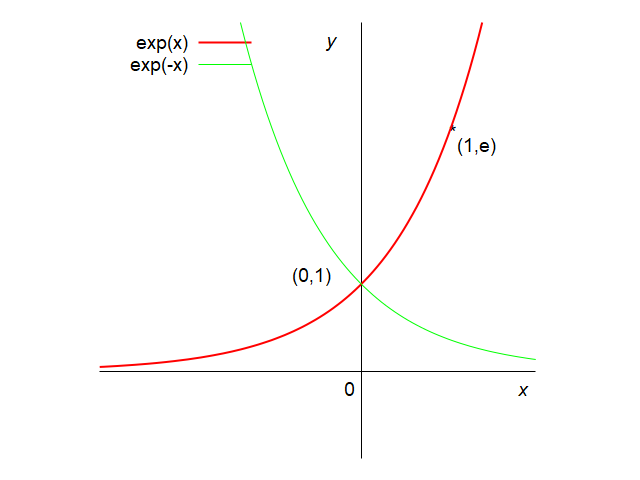
\includegraphics[width=\textwidth]{exp.png}
					\end{center}
				\end{minipage}
			\end{center}
			
			\qitem 指数関数と対数関数。
			\begin{center}
				\begin{minipage}{0.48\textwidth}
					\begin{itembox}[l]{指数関数と対数関数}
						\vspace{-3mm}
						\begin{align*}
							\textcolor{blue}{a}^{\textcolor{red}{x}} = \textcolor{green}{M} \Leftrightarrow \textcolor{red}{x}= \log_{\textcolor{blue}{a}} \textcolor{green}{M}
						\end{align*}
						\begin{itemize}
							\item 指数関数:\\底に\qbox{}を作用させて真数を求める関数
							\item 対数関数:\\真数は\qbox{}にどんな指数を与えたものかを求める関数
							\item \qbox{}に関して対称
						\end{itemize}
					\end{itembox}
				\end{minipage}
				\begin{minipage}{0.4\textwidth}
					\begin{center}
					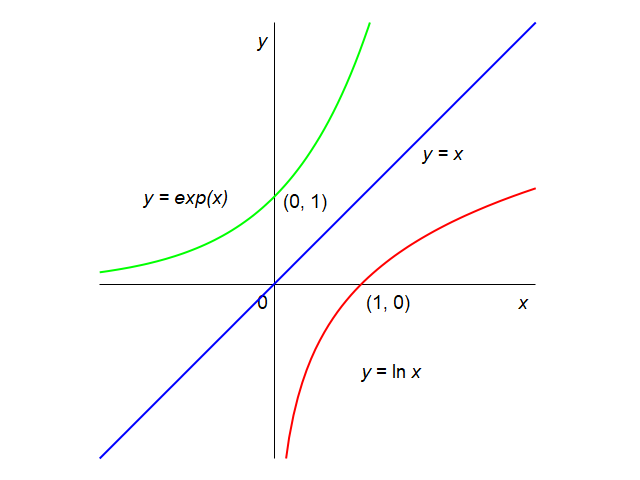
\includegraphics[width=\textwidth]{exp_ln.png}
					\end{center}
				\end{minipage}
			\end{center}

			\qitem 片対数グラフについて。
			\begin{center}
				\begin{minipage}{0.48\textwidth}
					\begin{itembox}[l]{片対数グラフの例}
						\begin{itemize}
							\item 指数関数を取り扱う際に、両辺の対数を取ると、\\
							$\ln y = ax + b$
							\begin{itemize}
								\item 関数値の\qbox{}が、
								\item 変数の\qbox{}となる。
								\item 指数が\qbox{}として求まる。
							\end{itemize}
						\end{itemize}
					\end{itembox}
				\end{minipage}
				\begin{minipage}{0.4\textwidth}
					\begin{center}
					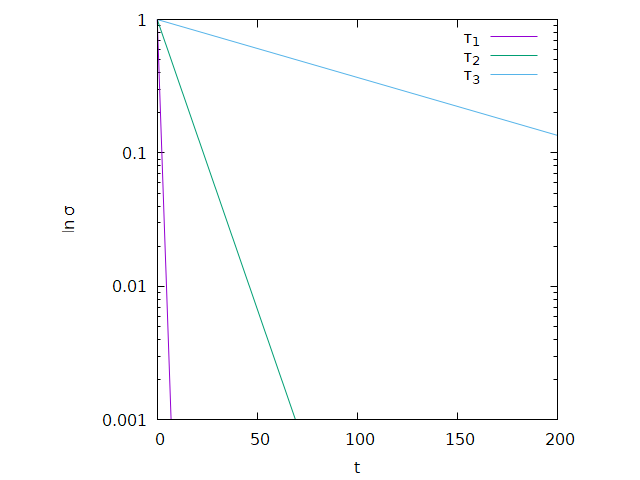
\includegraphics[width=\textwidth]{relux_6.png}
					\end{center}
				\end{minipage}
			\end{center}
		\end{qlist2}

		\begin{itembox}[l]{選択肢}
			\begin{center}
				\begin{tabular}{lllll}
					1. 底	&2. 1次関数	&3. 漸近線	&4. $y=x$	&5. 単調減少\\
					6. 指数	&7. 単調増加		&8. 対数				&9. 傾き
				\end{tabular}
			\end{center}
		\end{itembox}
\end{qlist}

\begin{itembox}[l]{解答}
    \begin{center} 
      \begin{tabular}{|c|c|c|c|c|c|c|c|c|} \hline
        (a) & (b) & (c) & (d) & (e) & (f) & (g) & (h) & (i)\\ \hline
        7 & 5 & 3 & 6 & 1 & 4 & 8 & 2 & 9 \\ \hline		
      \end{tabular}
    \end{center}
\end{itembox}

\begin{qlist}
	\qitem 微積分と微分方程式について、以下の\qbox{(j)}から\qbox{(q)}までのカッコを埋めてください。
		\begin{qlist2}
			\qitem 微分の直感的理解
			\begin{center}
				\begin{minipage}{0.48\textwidth}
					\begin{itembox}[l]{微分の直感的説明}
						\begin{itemize}
							\item 注目する点近傍での接線の\qbox{}
							\begin{itemize}
								\item 変数の増分と、
								\item \qbox{}との比をとる。
							\end{itemize}
							\item 変数の増分を\qbox{}にする。
						\end{itemize}
					\end{itembox}
				\end{minipage}
				\begin{minipage}{0.4\textwidth}
					\begin{center}
					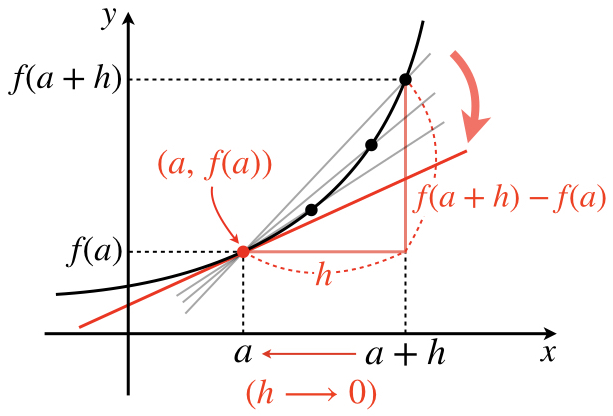
\includegraphics[width=\textwidth]{bibun.jpeg}
					\end{center}
				\end{minipage}
			\end{center}
	\qitem 微分方程式の解き方の例。
		\begin{itembox}[l]{一次反応を表す微分方程式}
			\textbf{1st step: }方程式の両辺に $\rmd t$ を掛ける。
			\begin{align*}
				\dfrac{1}{N} \mathrm{d}N= \qbox{}
			\end{align*}

			\textbf{2nd step: }方程式の両辺に積分記号 $\int$ をつける。
			\begin{align*}
				\int \dfrac{1}{N} \rmd N = \qbox{}
			\end{align*}

			\textbf{3rd step: }両辺の不定積分を計算する。
			\begin{align*}
				\qbox{} = -at + C_2
			\end{align*}

			\textbf{4th step: }積分定数を一つ($C=C_2-C_1$)にまとめる。
			\begin{align*}
				\ln N = -at + C
			\end{align*}

			\textbf{5th step: }指数関数に書き直してから、定数項を書き直し($C'=\exp(C)$)。
			\begin{align*}
				N= \qbox{} = \exp(C) \times \exp(-at) = C' \exp(-at)
			\end{align*}

			\textbf{6th step: }初期条件から、
			\begin{align*}
				&N(t=0) = C' \exp(-a*0) = N_0 \\
				\therefore\; &C' = N_0
			\end{align*}

			\textbf{Final step: }上記の定数項を用いて、濃度は時間の関数として以下となる。
			\begin{align*}
				N(t) = \qbox{}
			\end{align*}
	\end{itembox}
	\end{qlist2}
	\begin{itembox}[l]{選択肢}
		\begin{center}
			\begin{tabular}{llll}
				1. $\exp(-at + C)$	&2. $-a \int \mathrm{d} t$	&3. 無限小	&4. 傾き\\
				5. $\ln N +C_1$ &6. $-a\mathrm{d} t$	&7. 関数の増分	&8 $N_0 \exp(-at)$
			\end{tabular}
		\end{center}
	\end{itembox}
\end{qlist}

\begin{itembox}[l]{解答}
    \begin{center} 
      \begin{tabular}{|c|c|c|c|c|c|c|c|} \hline
        (j) & (k) & (l) & (m) & (n) & (o) & (p) & (q) \\ \hline
        4 & 7 & 3 & 6 & 2 & 5 & 1 & 8 \\ \hline		
      \end{tabular}
    \end{center}
\end{itembox}

\begin{qlist}
	\qitem 力学的な物理量について、以下の\qbox{(r)}から\qbox{(z)}までのカッコを埋めてください。
		\begin{qlist2}
			\qitem 仕事とエネルギーについて
			\begin{center}
				\begin{minipage}{0.42\textwidth}
					\begin{itembox}[l]{仕事とは}
						\begin{itemize}
							\item 質点に力を作用して、移動すること
							\item 仕事は、\qbox{} $F$ と移動した距離 $s$ の積
						\end{itemize}
							
\includegraphics[width=.8\textwidth]{work.png}
					\end{itembox}
				\end{minipage}
				\begin{minipage}{0.42\textwidth}
					\begin{itembox}[l]{エネルギーとは}
						\begin{itemize}
							\item 仕事をする\qbox{}のこと
							\item 物体や空間(場)は、その状態を変えることによりエネルギーを蓄える。
							\item 仕事とエネルギーの\qbox{}は同一。
						\end{itemize}
					\end{itembox}
				\end{minipage}
			\end{center}
			\qitem ポテンシャルについて
				\begin{itembox}[l]{ポテンシャルとは?}
					\begin{itemize}
						\item 基準の状態を定めて、
						\begin{itemize}
							\item 着目する状態にするために、その物体あるいは空間に加えた\qbox{}
						\end{itemize}
						\item 逆に言えば
						\begin{itemize}
							\item ある状態から基準の状態に戻るまでに、外に取り出すことのできる\qbox{}
						\end{itemize}
						\item 力が経路によらない\qbox{}であれば、ポテンシャルが位置のみの関数の状態量となる
					\end{itemize}
				\end{itembox}
			\qitem 摩擦と熱について
			\begin{center}
				\begin{minipage}{0.5\textwidth}
					\begin{itembox}[l]{摩擦と熱}
						\begin{itemize}
							\item 摩擦力は\qbox{}
								% \begin{itemize}
								% 	\item ポテンシャルは状態量ではなく経路に依存
								% \end{itemize}
							\item 内部の粒子の摩擦により、
								\begin{itemize}
									\item 粒子の運動エネルギーが増加し系全体の温度が\qbox{}
									\item 非断熱系では、熱エネルギーとして外界に散逸。
								\end{itemize}
							\item 非保存力も含めれば、系全体のエネルギーは\qbox{}
						\end{itemize}
					\end{itembox}
				\end{minipage}
				\begin{minipage}{0.34\textwidth}
					\begin{center}
					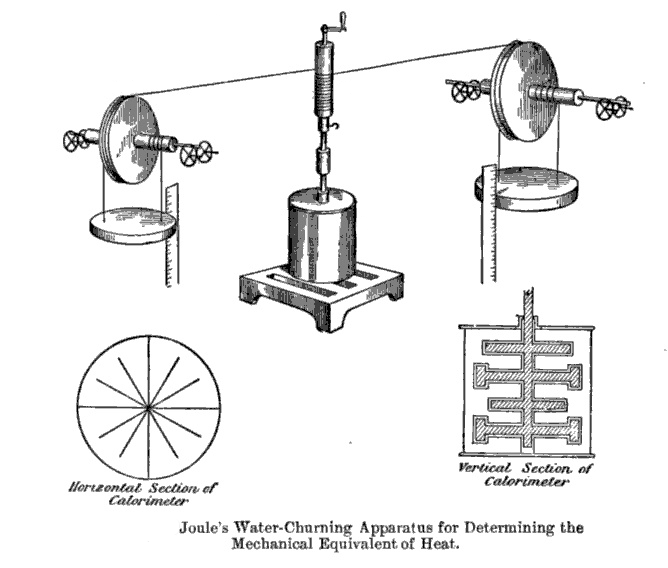
\includegraphics[width=\textwidth]{thermal_eng.png}
					\end{center}
				\end{minipage}
			\end{center}
		\end{qlist2}
	\begin{itembox}[l]{選択肢}
		\begin{center}
			\begin{tabular}{lllll}
				1. 非保存力	&2. 次元	&3. 上昇	&4. 仕事の量 &5. 保存力\\
				6. エネルギーの量	&7. 能力	&8 作用させた力 &9. 保存
			\end{tabular}
		\end{center}
	\end{itembox}
\end{qlist}

\begin{itembox}[l]{解答}
    \begin{center} 
      \begin{tabular}{|c|c|c|c|c|c|c|c|c|} \hline
        (r) & (s) & (t) & (u) & (v) & (w) & (x) & (y) & (z) \\ \hline
        8 & 7 & 2 & 4 & 6 & 5 & 1 & 3 & 9 \\ \hline		
      \end{tabular}
    \end{center}
\end{itembox}

\end{document}